\subsubsection*{Hacker A20-20L}

\begin{table}[h!]
	\centering
	\begin{tabular}{l l l l}
		RC-Parameter & & & \\ \hline
			& Kühlung	& & Mittelmässig \\
			& Batterie	& & LiPo 10Ah, voll, 3S1P, 3.7V \\
			& Regler	& & 30A \\
			& Propeller	& & $\o=10"$, $p=5"$, $b=2$, $p_c=1.3$, $g_r=1$ \\
			& & & \\
		Resultate (max.) & & & \\ \hline
			& Motorstrom	& $I$	& 21.2 A \\
			& Motorspannung	& $U$	& 11.5 V \\
			& Drehzahl	& $n$	& 9111 min$^{-1}$ \\
			& Leistung 	& $P_e$	& 243.8 W \\
			&		& $P_m$	& 186.4 W \\
			& Wikungsgrad	& $\eta$& 76.5 \% \\
			& Motortemperatur
					& $T$	& 56 C \\
			& & & \\
		Berechnungen & & & \\ \hline
			& Winkelgeschwindigkeit
					& $\omega_m$	& 954.1 s$^{-1}$ \\
			& Drehmoment	& $M$		& 0.195 Nm
	\end{tabular}
	\caption{Simulationsdaten des Hacker A20-20L}
\end{table}

\begin{figure}[h!]
	\centering
	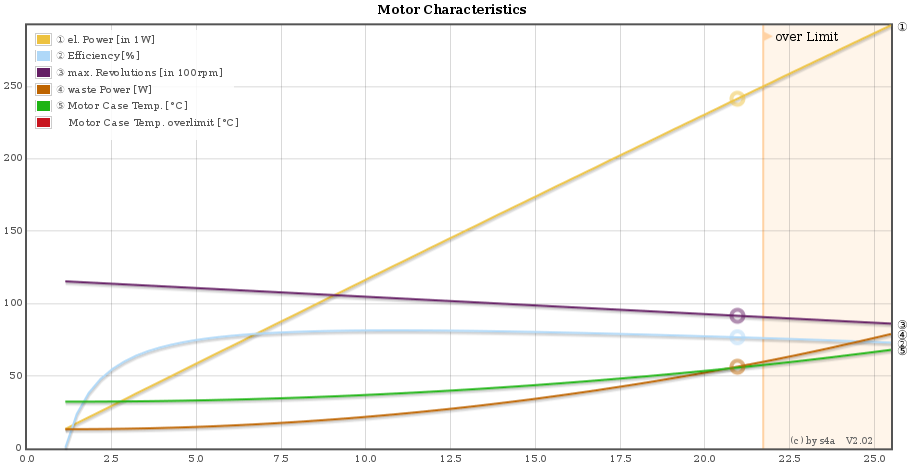
\includegraphics[width=1\textwidth]{../../fig/motor/ecalc_A20-20L.png}
	\caption{Berechnete Kennlinien des Hacker A20-20L}
	\label{fig:ecalc_A20-20L}
\end{figure}
